\section{DAO - \emph{Data Acceso Object}}

\begin{frame}{DAO - \emph{Data Acceso Object}}
	\begin{itemize}
		\item DAO Es un patrón de diseño del tipo creacional.
		\item Est\'a basado directamente en el concepto de \emph{Separaci\'on de Responsabilidades}.
		\begin{block}{Separaci\'on de Responsabilidades.}
		\begin{itemize}
			\item Cada clase es creada bajo un \'unico fin o responsabilidad asignada.
			\item La responsabilidad debe ser cumplida en su totalidad por la clase.
			\item Este concepto define que una responsabilidad debe estar asociado de forma directa a solo un clase.
		\end{itemize}
		\end{block}
	\end{itemize}

\end{frame}

\begin{frame}{DAO - Responsabilidad}
	\begin{itemize}
		\item En una aplicación empresarial, DAO tiene la responsabilidad de separar la persistencia de datos del resto de funcionalidades.
		\item Esto proporciona \emph{independencia de la fuente de datos}, al tener dicha responsabilidad encapsulada dentro de la misma clase.
		\begin{block}{Nota Relevante}
		\begin{itemize}
			\item Un principio b\'asico de un buen diseño de sistema es identificarlos aspectos de la aplicacion
						que cambian o pueden cambiar y separarlos de los que van a permanecer siempre fijos. Muchos patrones de diseño se basan en encapsular de alguna forma
						la parte que cambia para hacer mas f\'acil la extensi\'on del sistema.
			\item DAO encapsula la parte que puede cambiar, que es la interacci\'on con la fuente de datos.
		\end{itemize}
		\end{block}
	\end{itemize}

\end{frame}

%\begin{frame}{Tips - Ocultamiento de Informaci\'on - Ejemplo.}
  %\begin{figure}
    %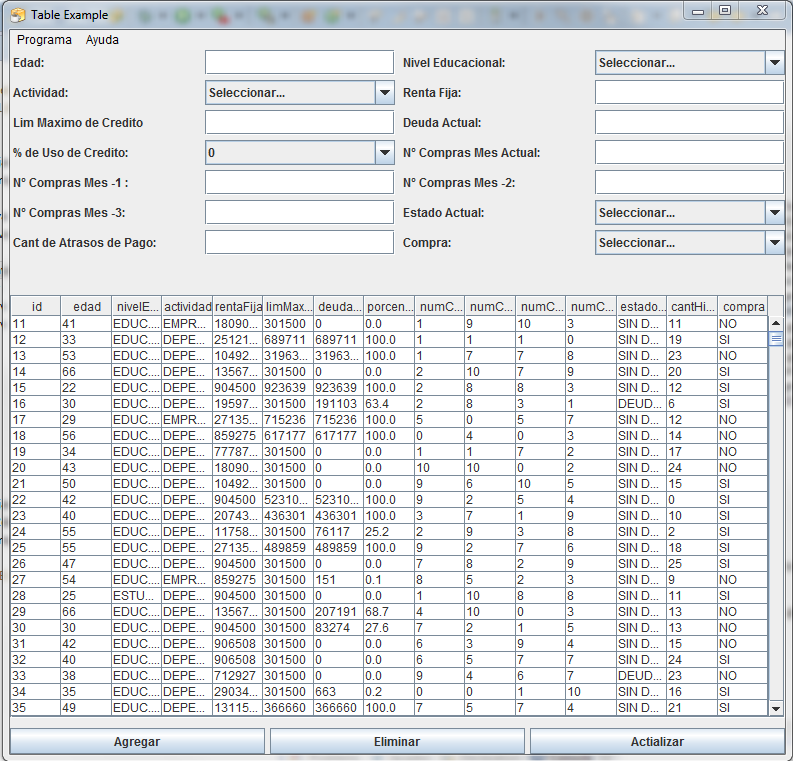
\includegraphics[scale=0.3]{figuras/DT.PNG}
  %\end{figure}
%\end{frame}

%\begin{frame}{Manejo de Excepciones - try, catch, finally}
%\begin{block}{Ejemplo.}
%\lstinputlisting[language=Java,caption={},numbers=none]{resources/excepciones/Finally.java}
%\end{block}
%\end{frame}
